

This stone tackles the Rayleigh-Taylor instability problem of van Keken \etal \cite{vaks97}. 
It builds on Stone 93 as it relies on Crouzeix-Raviart elements and Delaunay meshes
generated by the Triangle code \cite{shew14}.  

However, this code does implements mesh adaptation and the python code then calls the Triangle mesher code
at every timestep (the remeshing cost is negligible).
I unfortunately cannot prevent Triangle from adding nodes in between the interface nodes, thereby 
ruining the numbering and the flagging of these nodes. I have therefore implemented a refinement 
process which add nodes on the interface when two consecutive nodes are getting too far apart. 


\begin{center}
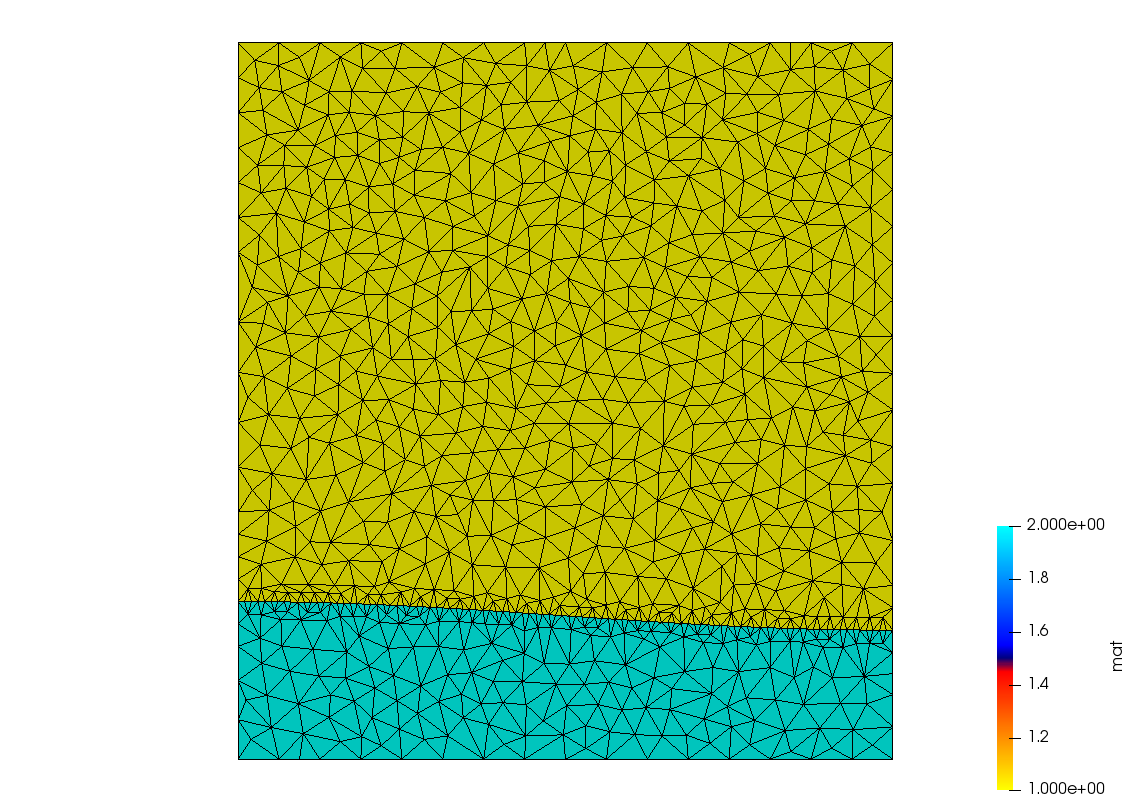
\includegraphics[width=5.5cm]{python_codes/fieldstone_95/init/mat}
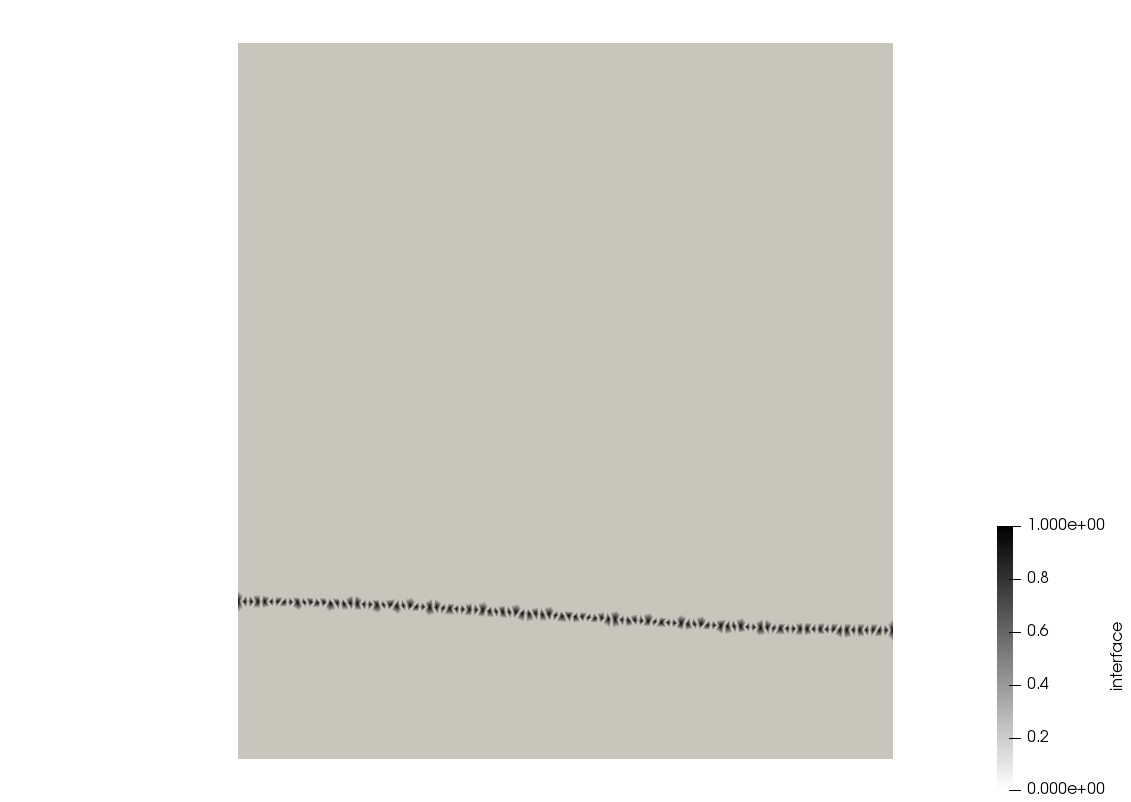
\includegraphics[width=5.5cm]{python_codes/fieldstone_95/init/interface}
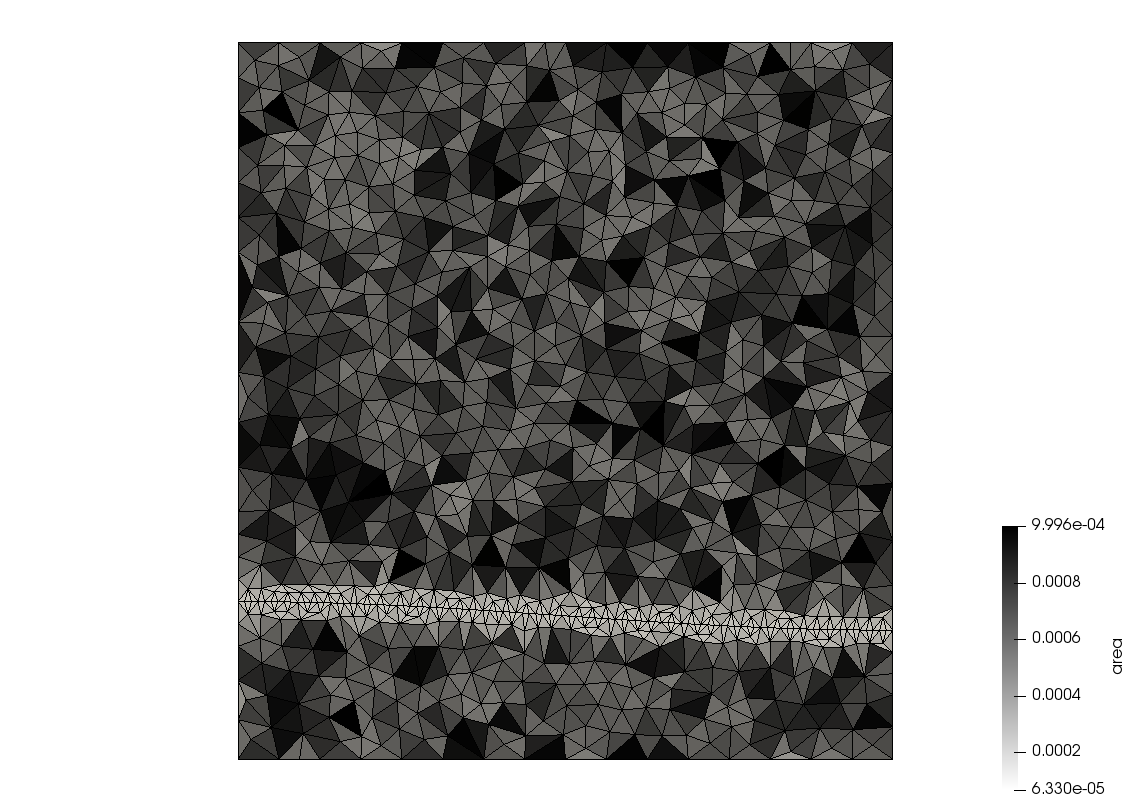
\includegraphics[width=5.5cm]{python_codes/fieldstone_95/init/area}\\
{\captionfont Interface counts 100 points, Triangle argument a=0.001, } 
\end{center}

The number of parameters one can vary is somewhat limited:
\begin{itemize}
\item the CFL number - default 0.25 (note that the time step is limited to 0.5)
\item the maximum area $a$ of triangles (passed as argument to Triangle) - default 0.001
\item the initial number of triangle vertices on the interface $np_{surf}$ - default 100
\item the stretch factor controlling the addition of points $\gamma$ - default 1.5
\end{itemize}

In the end we wish to plot the time evolution of the root mean square velocity and 
establish the time and amplitude of the first two peaks. We also wish to control 
for volume conservation 


\begin{center}
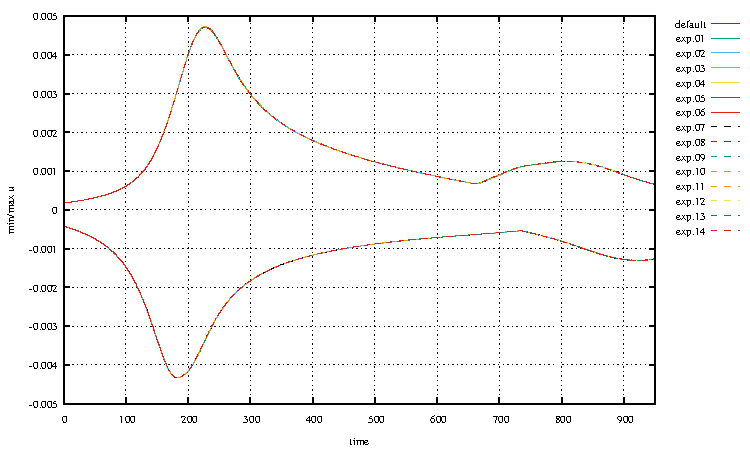
\includegraphics[width=5.5cm]{python_codes/fieldstone_95/results/u}
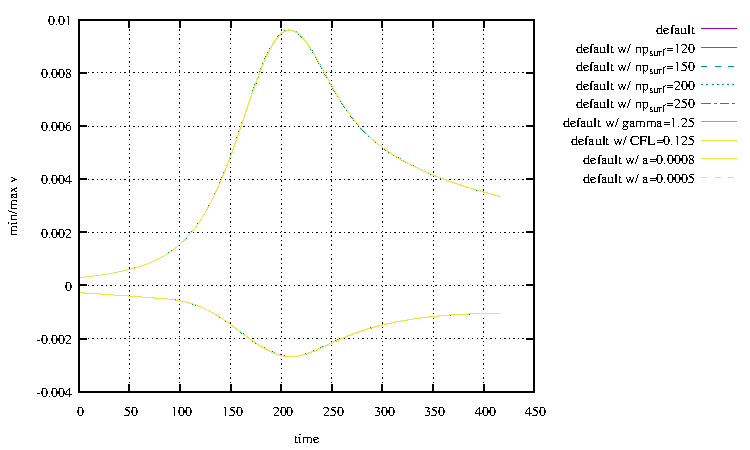
\includegraphics[width=5.5cm]{python_codes/fieldstone_95/results/v}\\
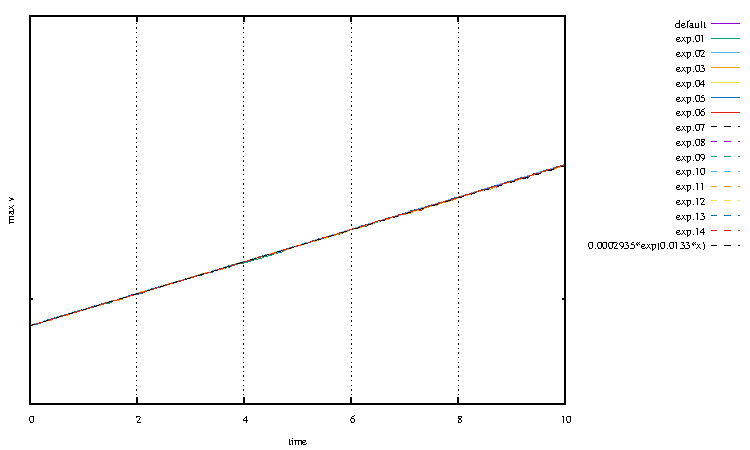
\includegraphics[width=5.5cm]{python_codes/fieldstone_95/results/v_start}
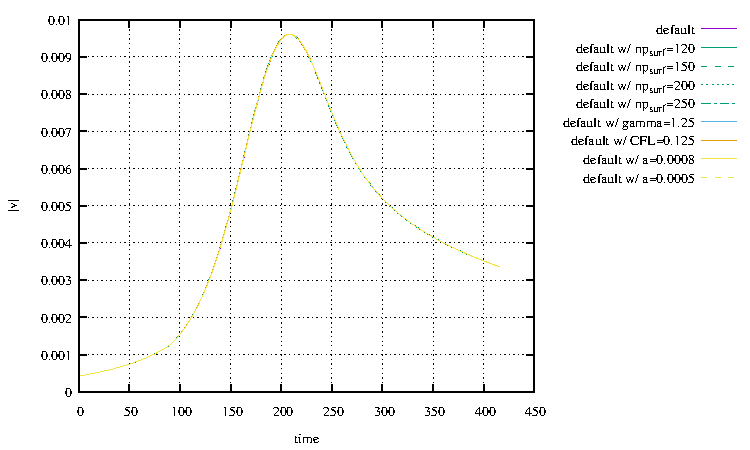
\includegraphics[width=5.5cm]{python_codes/fieldstone_95/results/vel}\\
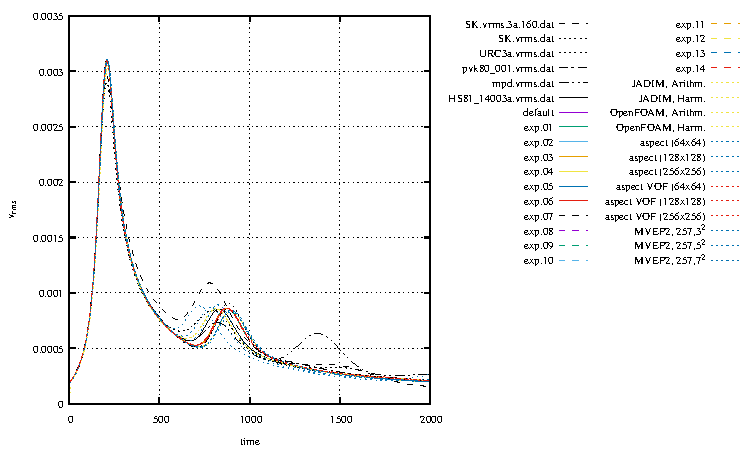
\includegraphics[width=5.5cm]{python_codes/fieldstone_95/results/vrms2000}
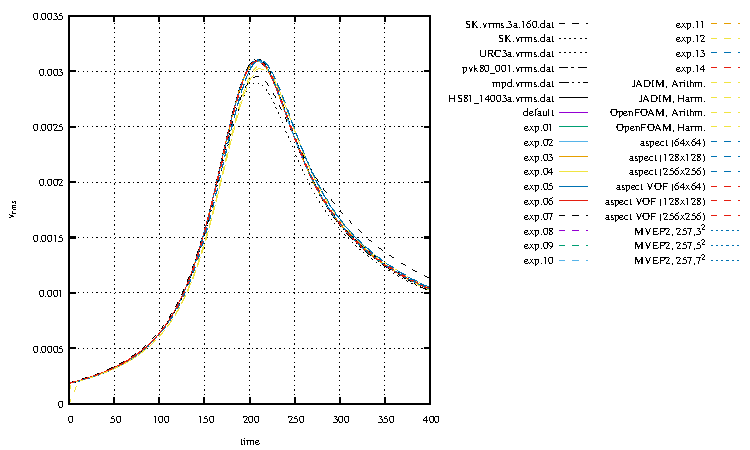
\includegraphics[width=5.5cm]{python_codes/fieldstone_95/results/vrms400}
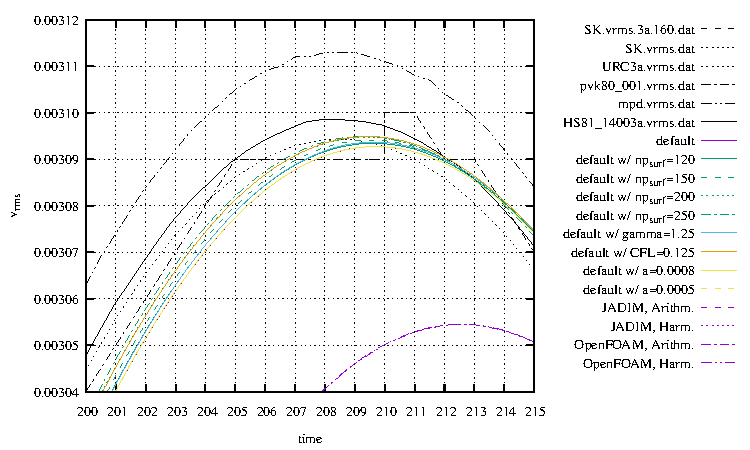
\includegraphics[width=5.5cm]{python_codes/fieldstone_95/results/vrms_peak1}\\
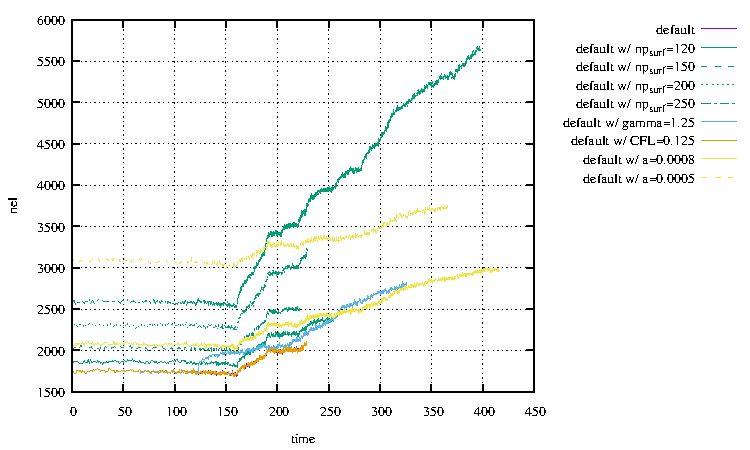
\includegraphics[width=5.5cm]{python_codes/fieldstone_95/results/nel}
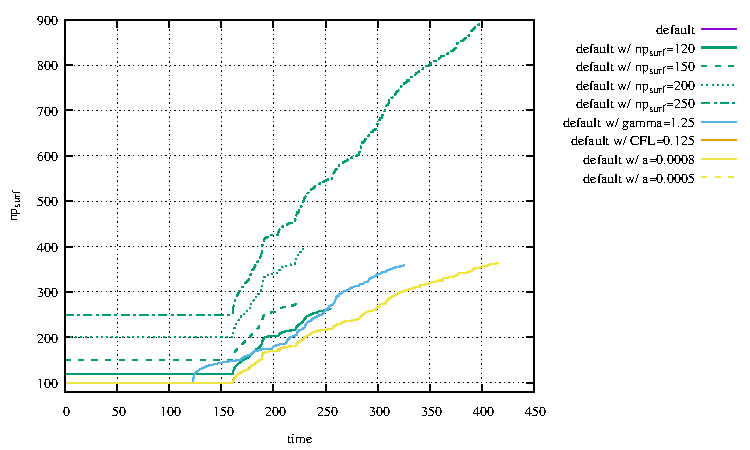
\includegraphics[width=5.5cm]{python_codes/fieldstone_95/results/np_surf}\\
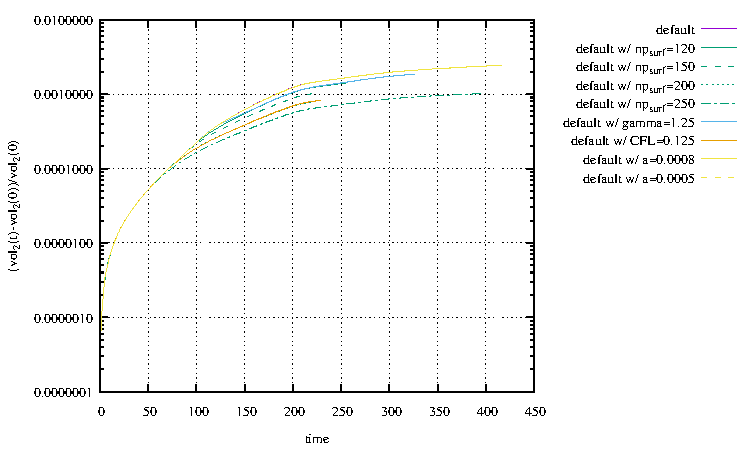
\includegraphics[width=5.5cm]{python_codes/fieldstone_95/results/vol2}
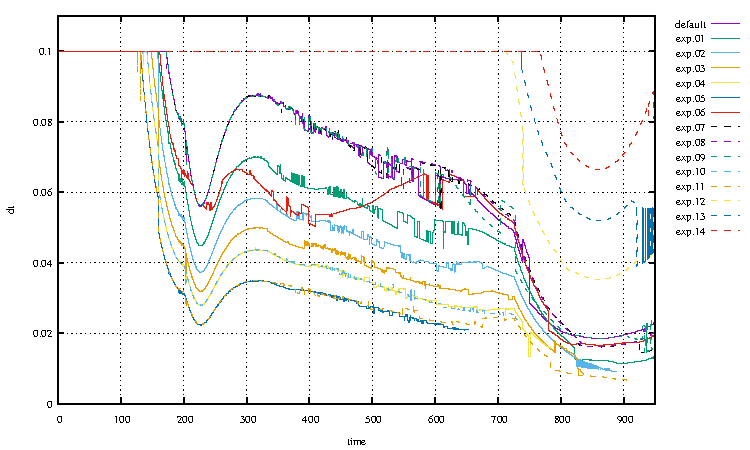
\includegraphics[width=5.5cm]{python_codes/fieldstone_95/results/dt}
\end{center}


\begin{center}
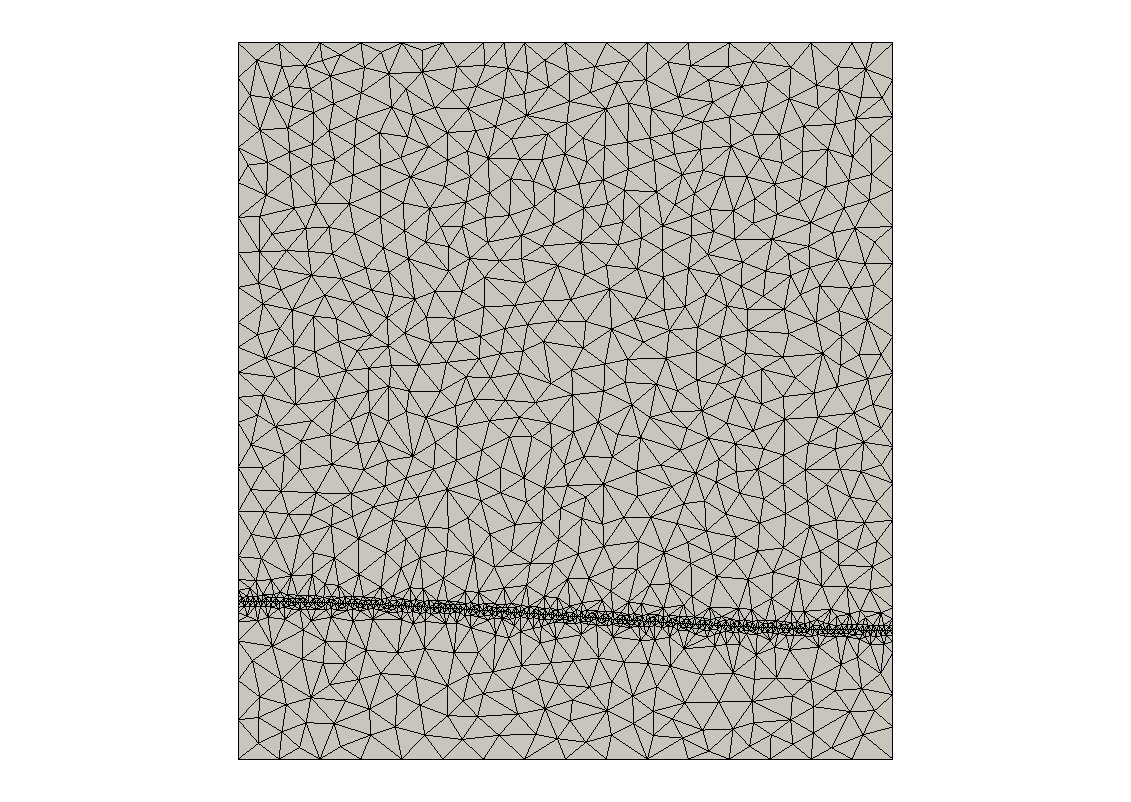
\includegraphics[width=5.5cm]{python_codes/fieldstone_95/results/npsurf250/grid0000.png}
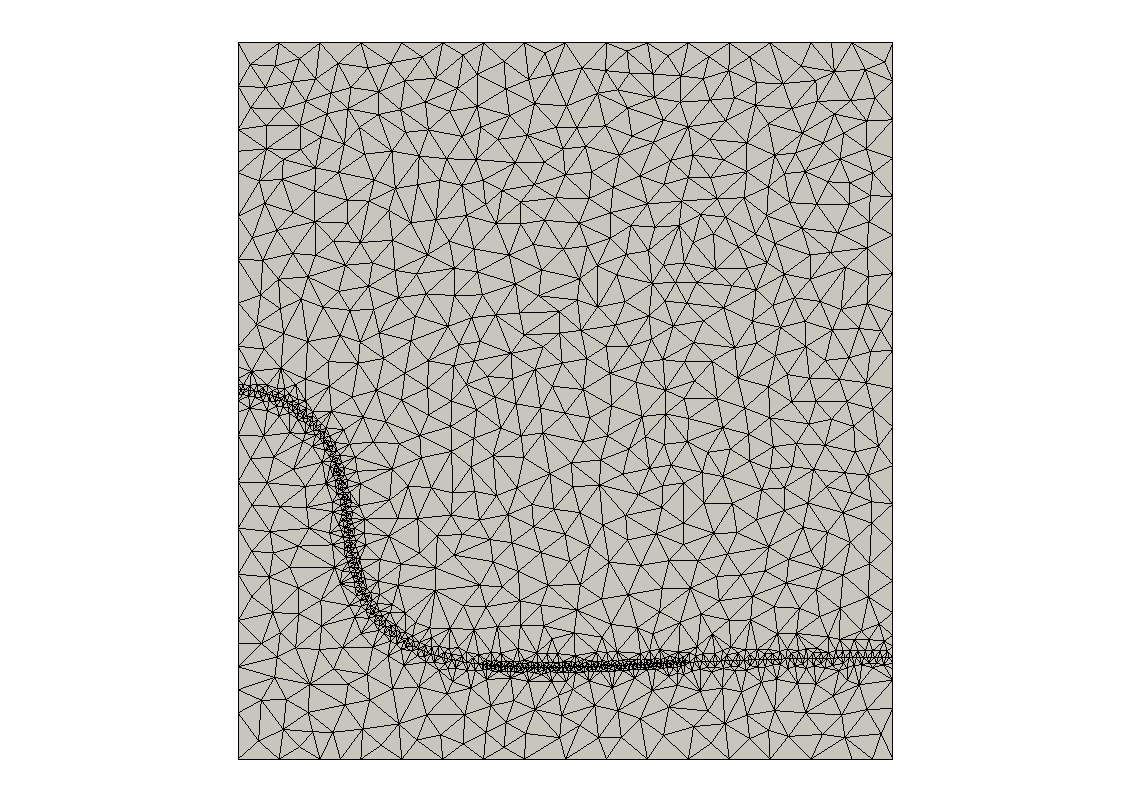
\includegraphics[width=5.5cm]{python_codes/fieldstone_95/results/npsurf250/grid0050.png}
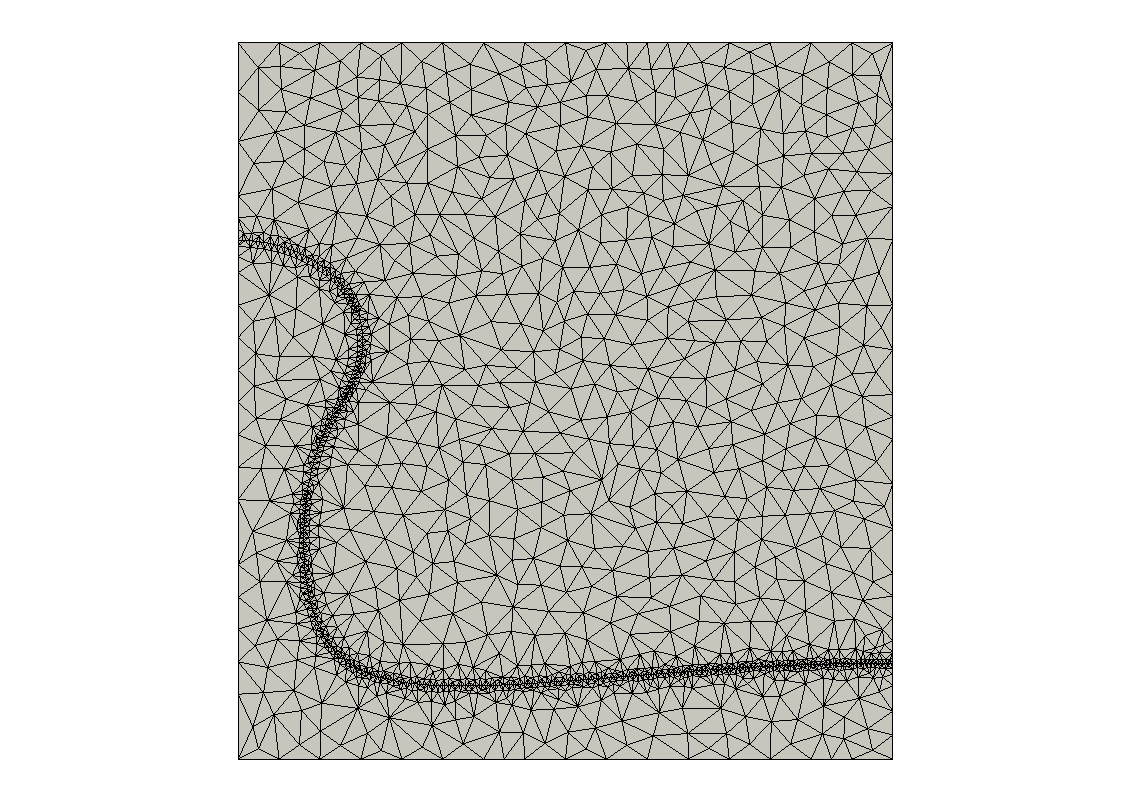
\includegraphics[width=5.5cm]{python_codes/fieldstone_95/results/npsurf250/grid0100.png}\\
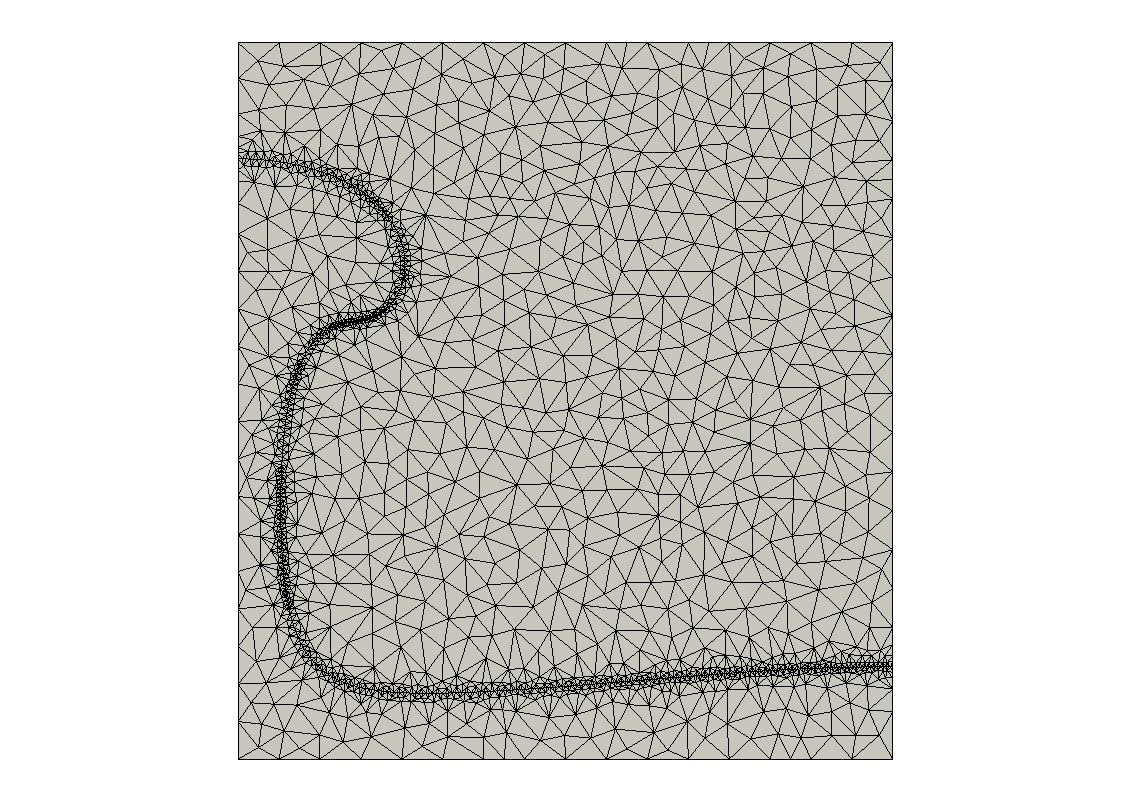
\includegraphics[width=5.5cm]{python_codes/fieldstone_95/results/npsurf250/grid0150.png}
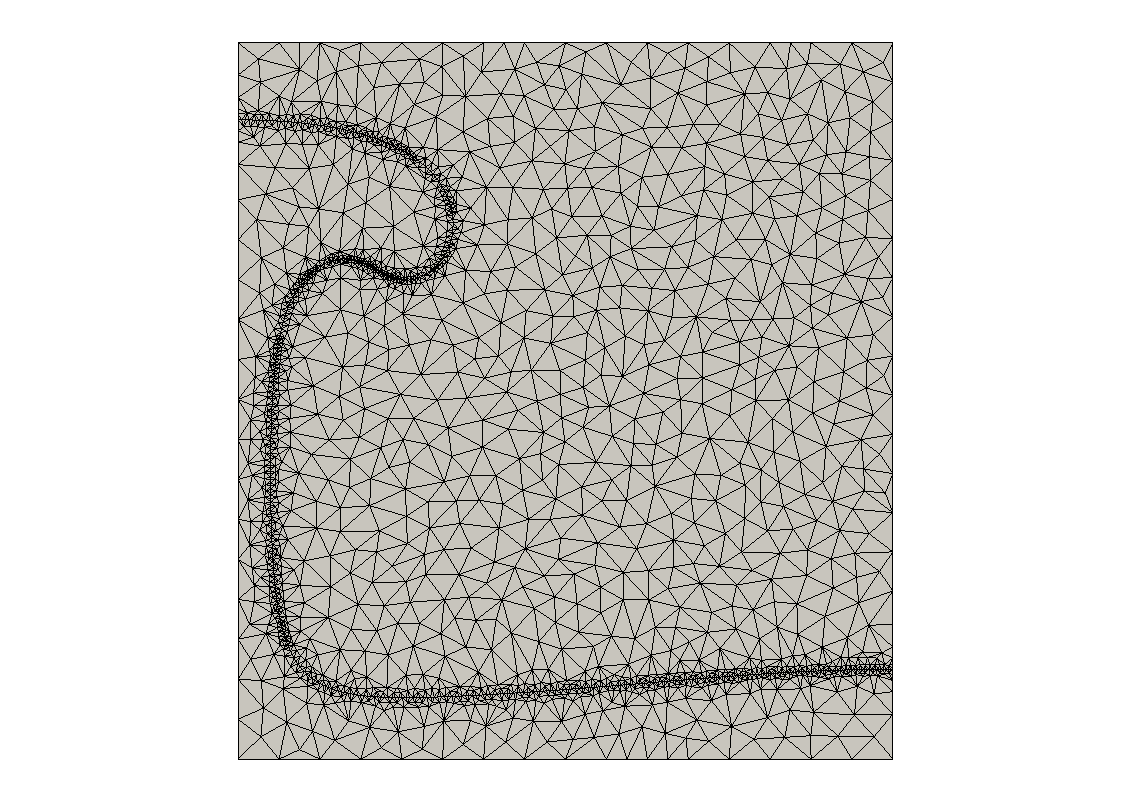
\includegraphics[width=5.5cm]{python_codes/fieldstone_95/results/npsurf250/grid0200.png}
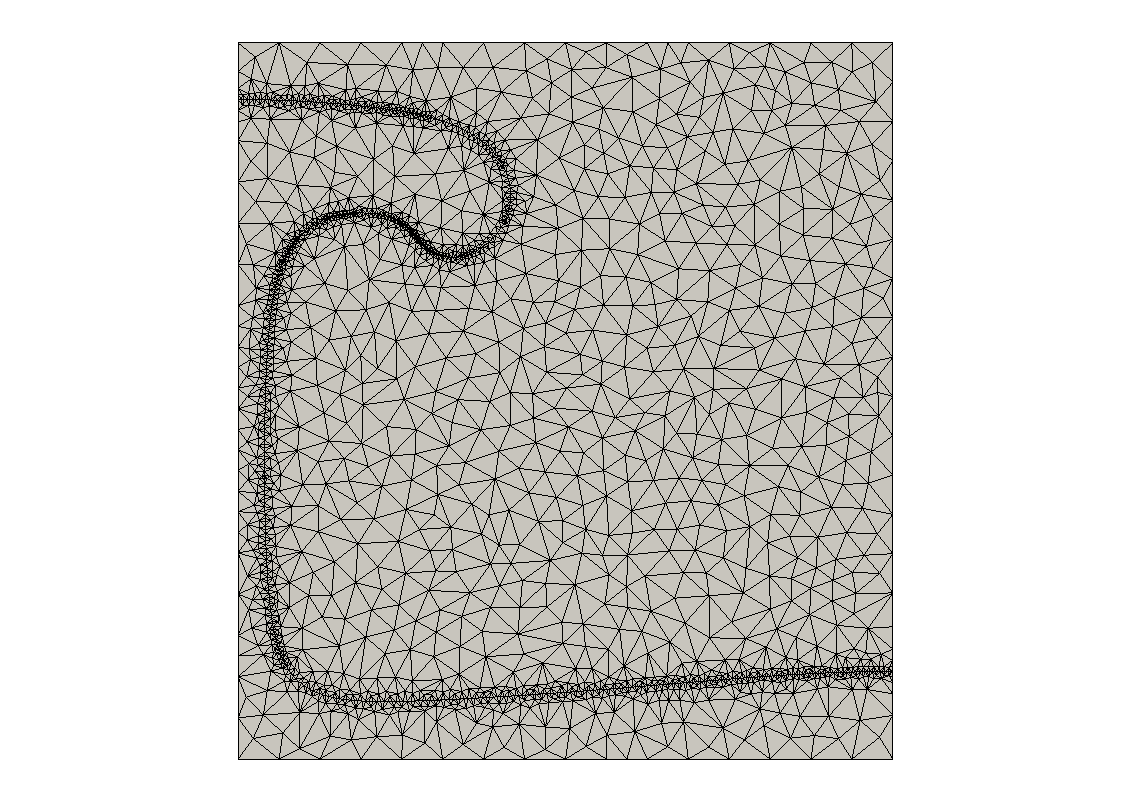
\includegraphics[width=5.5cm]{python_codes/fieldstone_95/results/npsurf250/grid0250.png}\\
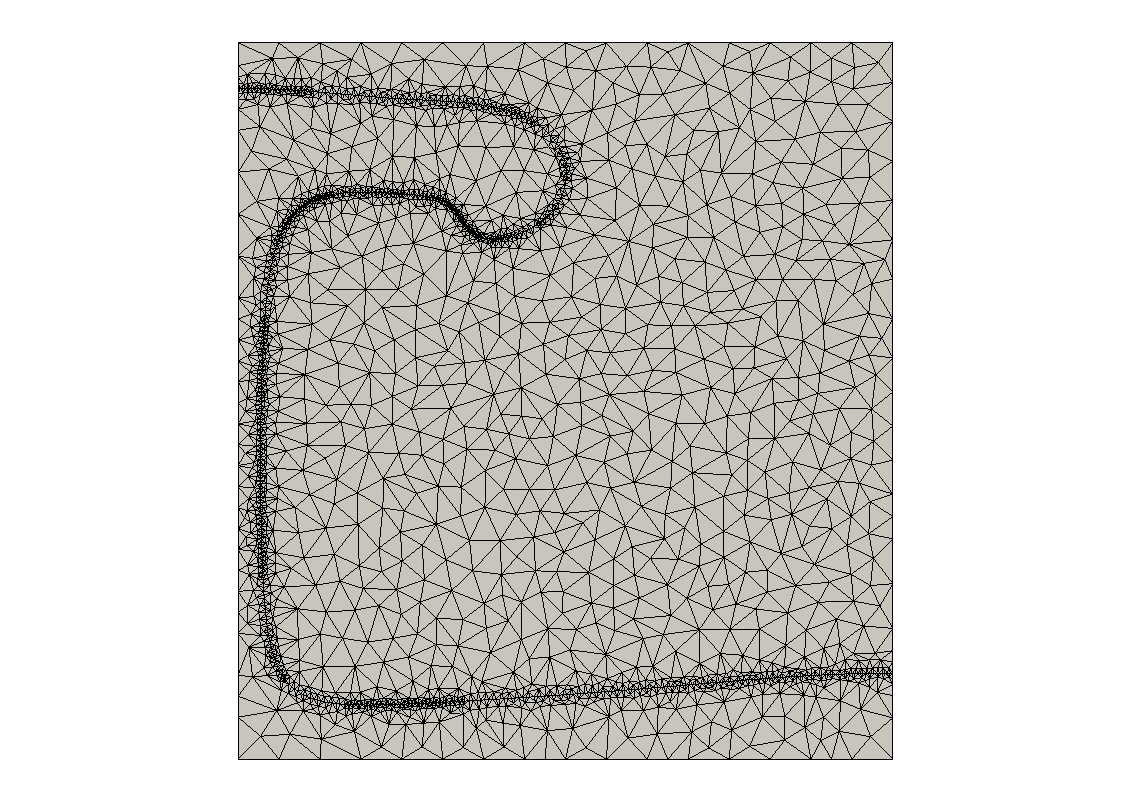
\includegraphics[width=5.5cm]{python_codes/fieldstone_95/results/npsurf250/grid0300.png}
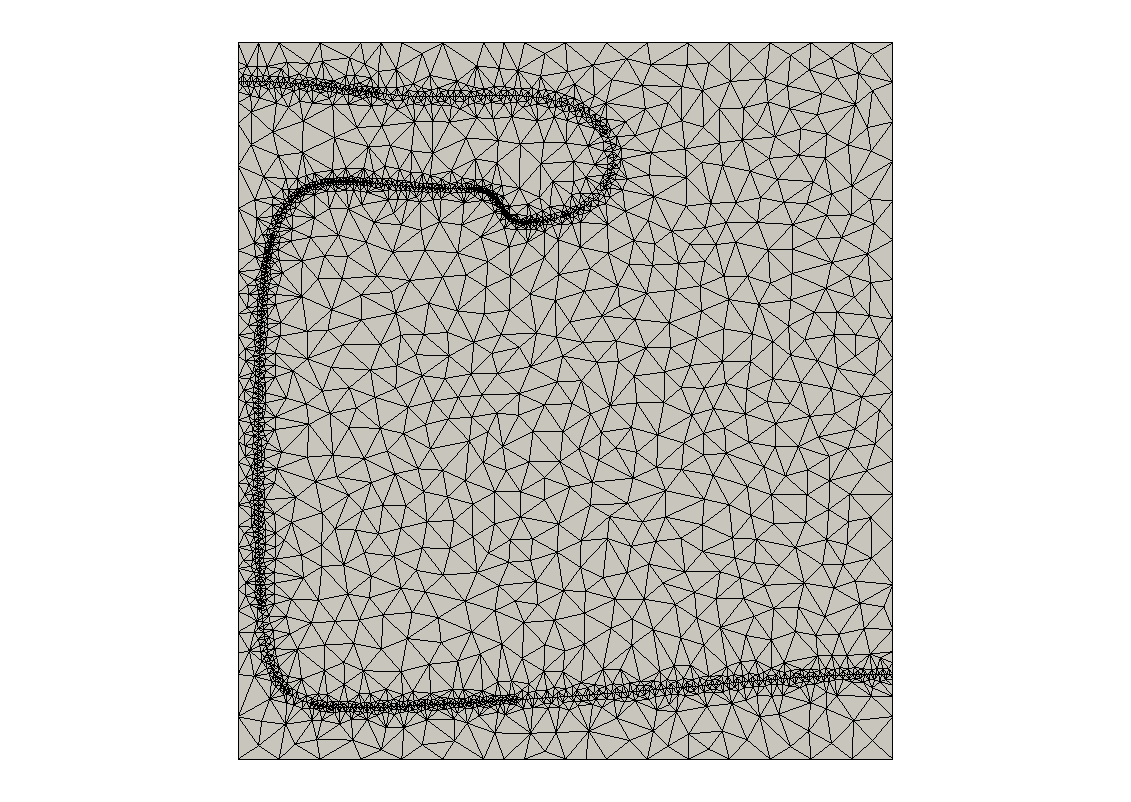
\includegraphics[width=5.5cm]{python_codes/fieldstone_95/results/npsurf250/grid0350.png}
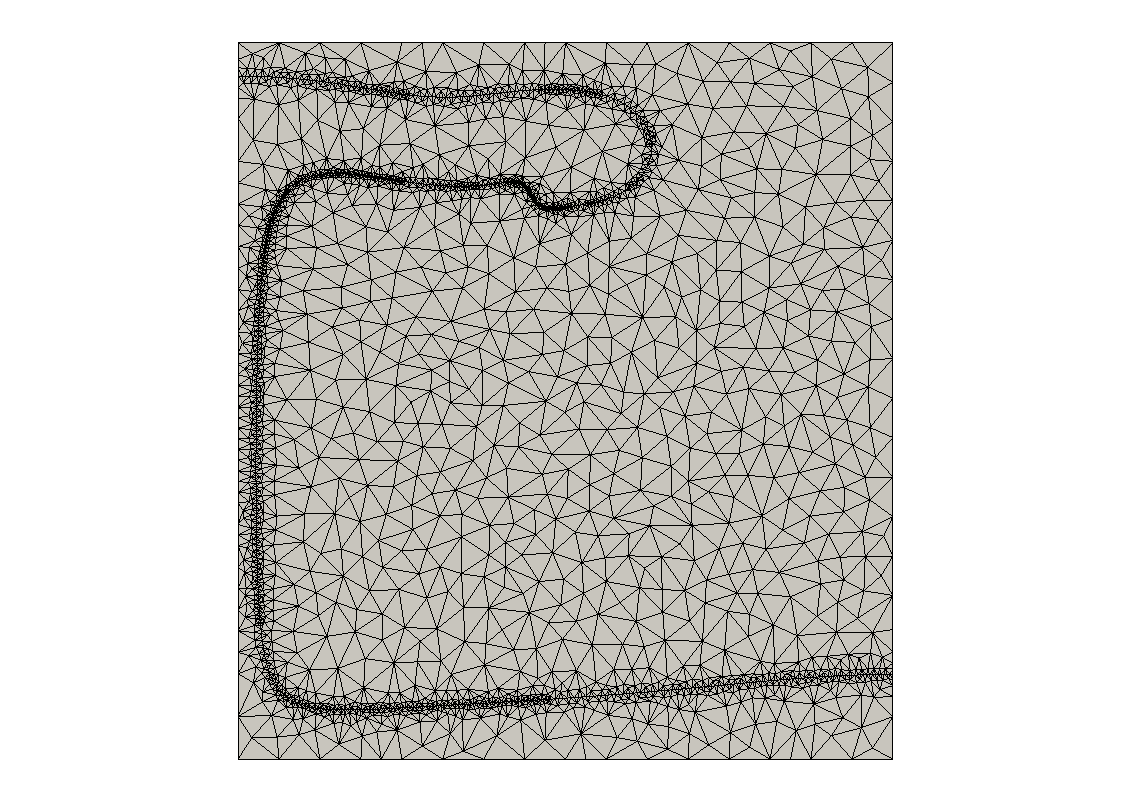
\includegraphics[width=5.5cm]{python_codes/fieldstone_95/results/npsurf250/grid0400.png}\\
{\captionfont Cade default + npsurf=250, up to time = 400}
\end{center}


\begin{center}
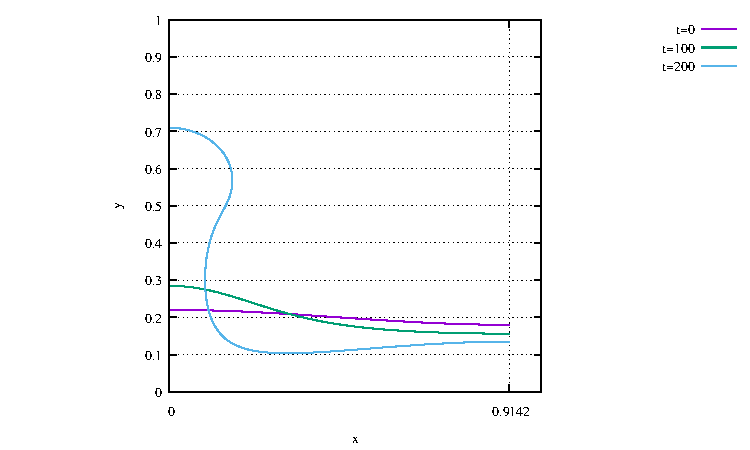
\includegraphics[width=8cm]{python_codes/fieldstone_95/results/interface.pdf}\\
{\captionfont position of the material interface as a function of time. Default case.}
\end{center}


I have also plotted the vrms against those of the original paper and those of Louis-Napoleon \etal \cite{logb20}
(with codes JADIM and OpenFOAM). 
The main parameter which seems to govern overal mass/volume conservation is the resolution of the interface. 

QUESTION: at the end of the first time step, when I write down the time associated with the measurements, should I write 0
or dt ?

QUESTION: does reduced density use change results ?

TODO: run until time=1500

TODO: viscosity ratio 10 and 100 cases

